\begin{center}
    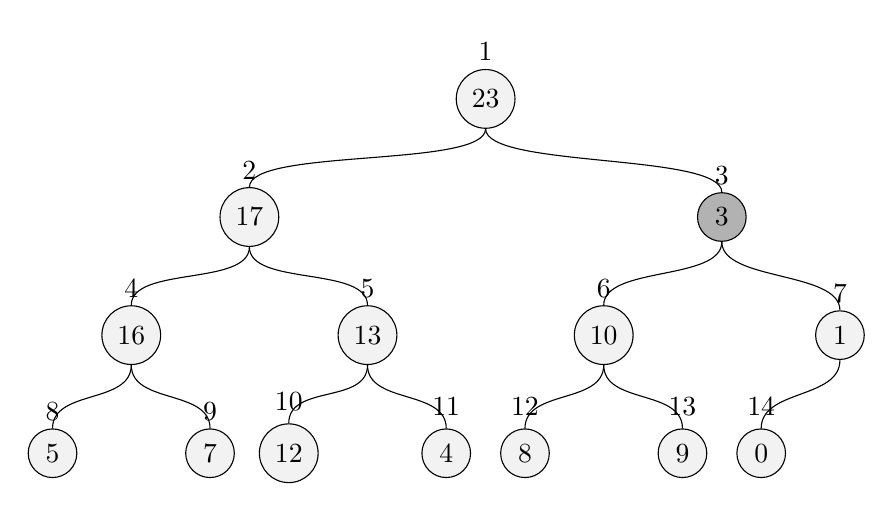
\begin{tikzpicture}[
       edge from parent path=
    {(\tikzparentnode.south) .. controls +(0,-.5) and +(0,.5)
                             .. (\tikzchildnode.north)},
    level 1/.style={sibling distance=6cm}, 
    level 2/.style={sibling distance=3cm},                        
    level 3/.style={sibling distance=2cm},                         
    level 4/.style={sibling distance=1cm},
   every node/.style={draw, circle, fill=gray, fill opacity=0.1, text opacity=1},
   label distance=-1mm]
   
\node[label=90:$1$] {23}
    child {node[label=90:$2$] {17}
        child {node[label=90:$4$] {16}
            child {node[label=90:$8$] {5}}
            child {node[label=90:$9$] {7}}
        }
        child {node[label=90:$5$] {13}
            child {node[label=90:$10$] {12}}
            child {node[label=90:$11$] {4}}
            }
    }
    child {node[label=90:$3$, fill=black, fill opacity=0.3] {3}
        child {node[label=90:$6$] {10}    
            child {node[label=90:$12$] {8}}
            child {node[label=90:$13$] {9}}
        }
        child {node[label=90:$7$] {1}
            child {node[label=90:$14$] {0}}
            child[missing] {}
        }
    };

\end{tikzpicture}
\end{center}

\begin{center}
    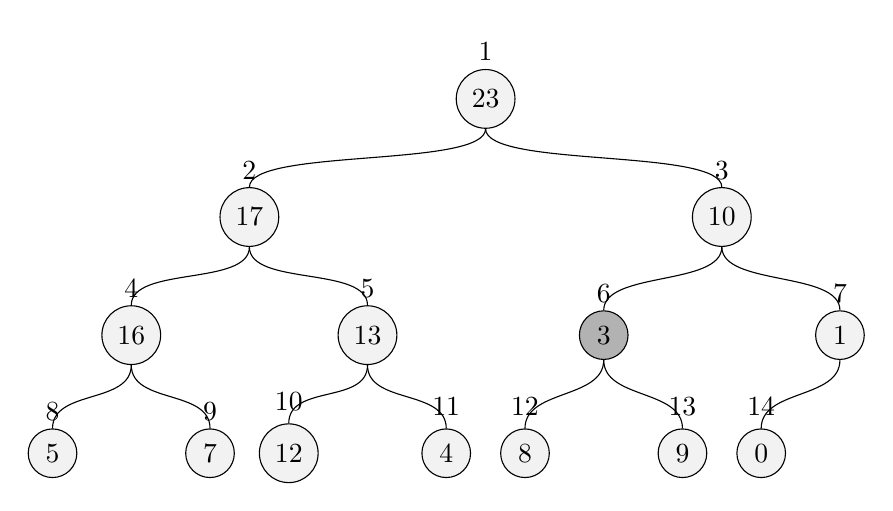
\begin{tikzpicture}[
       edge from parent path=
    {(\tikzparentnode.south) .. controls +(0,-.5) and +(0,.5)
                             .. (\tikzchildnode.north)},
    level 1/.style={sibling distance=6cm}, 
    level 2/.style={sibling distance=3cm},                        
    level 3/.style={sibling distance=2cm},                         
    level 4/.style={sibling distance=1cm},
   every node/.style={draw, circle, fill=gray, fill opacity=0.1, text opacity=1},
   label distance=-1mm]
   
\node[label=90:$1$] {23}
    child {node[label=90:$2$] {17}
        child {node[label=90:$4$] {16}
            child {node[label=90:$8$] {5}}
            child {node[label=90:$9$] {7}}
        }
        child {node[label=90:$5$] {13}
            child {node[label=90:$10$] {12}}
            child {node[label=90:$11$] {4}}
            }
    }
    child {node[label=90:$3$] {10}
        child {node[label=90:$6$, fill=black, fill opacity=0.3] {3}    
            child {node[label=90:$12$] {8}}
            child {node[label=90:$13$] {9}}
        }
        child {node[label=90:$7$] {1}
            child {node[label=90:$14$] {0}}
            child[missing] {}
        }
    };

\end{tikzpicture}
\end{center}

\begin{center}
    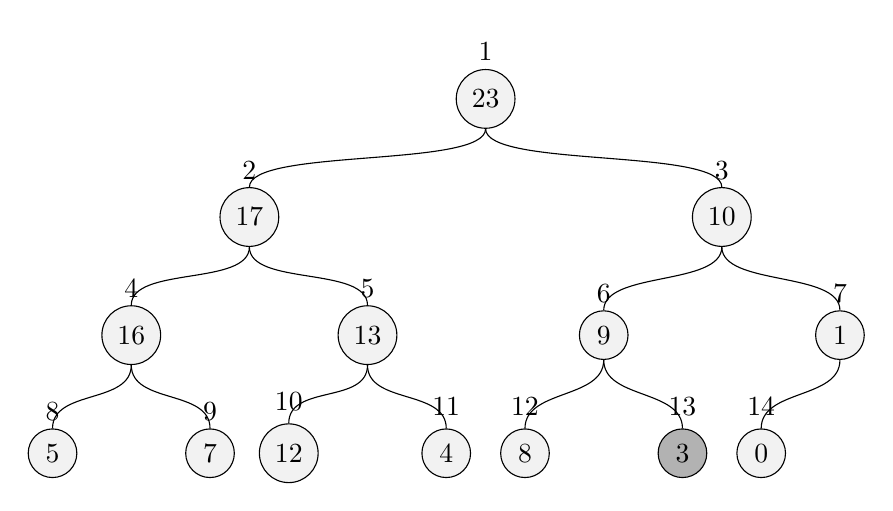
\begin{tikzpicture}[
       edge from parent path=
    {(\tikzparentnode.south) .. controls +(0,-.5) and +(0,.5)
                             .. (\tikzchildnode.north)},
    level 1/.style={sibling distance=6cm}, 
    level 2/.style={sibling distance=3cm},                        
    level 3/.style={sibling distance=2cm},                         
    level 4/.style={sibling distance=1cm},
   every node/.style={draw, circle, fill=gray, fill opacity=0.1, text opacity=1},
   label distance=-1mm]
   
\node[label=90:$1$] {23}
    child {node[label=90:$2$] {17}
        child {node[label=90:$4$] {16}
            child {node[label=90:$8$] {5}}
            child {node[label=90:$9$] {7}}
        }
        child {node[label=90:$5$] {13}
            child {node[label=90:$10$] {12}}
            child {node[label=90:$11$] {4}}
            }
    }
    child {node[label=90:$3$] {10}
        child {node[label=90:$6$] {9}    
            child {node[label=90:$12$] {8}}
            child {node[label=90:$13$, fill=black, fill opacity=0.3] {3}}
        }
        child {node[label=90:$7$] {1}
            child {node[label=90:$14$] {0}}
            child[missing] {}
        }
    };

\end{tikzpicture}
\end{center}